\section{Energy scale calibration}

\subsection{Resolution Scans}
\label{sec:resolution_scans}
As the signal from the detector is rather weak, the detector is connected to an
amplifying circuit as described in Sect.~\ref{sec:calibration:set-up}. However
there is a trade-off associated with this procedure as amplification also
applies to noise in the detector. In order to increase the signal strength the
voltage applied to the detector can be increased which in turn increases the
amount of signal electrons and leads to a stronger output signal. Along with
this comes though an increased probability for spontaneous discharges along
impurities and dirt remaining in the detector despite extensive cleaning
procedures as described in Sec.~\ref{sec:construction}.

As the two possibilities for varying the output signal strength are associated
with independent increases of noise and accordingly reduction of resolution we
are performing resolution scans for the two samples we are interested in
measuring: Americium and iron.

In order to reliably determine the resolution a Gaussian is fitted to the sample
peak previously identified in the multi-channel analyser (MCA) spectrum. We look
at the variable peak width divided by the peak position in order to determine
the resolution of our peak. For the peak width we are using the full-width
half-maximum (FWHM) value. As secondary decays will affect especially the lower
end of the decay Gaussian \todo[inline]{how are they called exactly? secondary seems
  wrong} shape we are defining regions of interest (ROI) in which the Gaussian
is fitted.

The spectra obtained for americium (Fig \ref{fig:scan:americium}) and iron
(Fig. \ref{fig:scan:iron}) are presented in appendix~\ref{app:resolution-scans} for different gains and voltages.
A Gaussian is fitted to the marked ROI (blue lines) and the obtained channel number as well as
full-width half-maximum (FWHM) in channels are denoted in each figure.

The obtained parameters from the fit are plotted in Fig.
\ref{fig:resolution:americium} and \ref{fig:resolution:iron} for americium and
iron respectively. The uncertainties are propagated from the fit. Additionally to the
total uncertainty on the FWHM, a \SI{10}{\percent} systematic
uncertainty was added due to the dependency on choosing the corresponding ROI.

\begin{figure}[htb]
  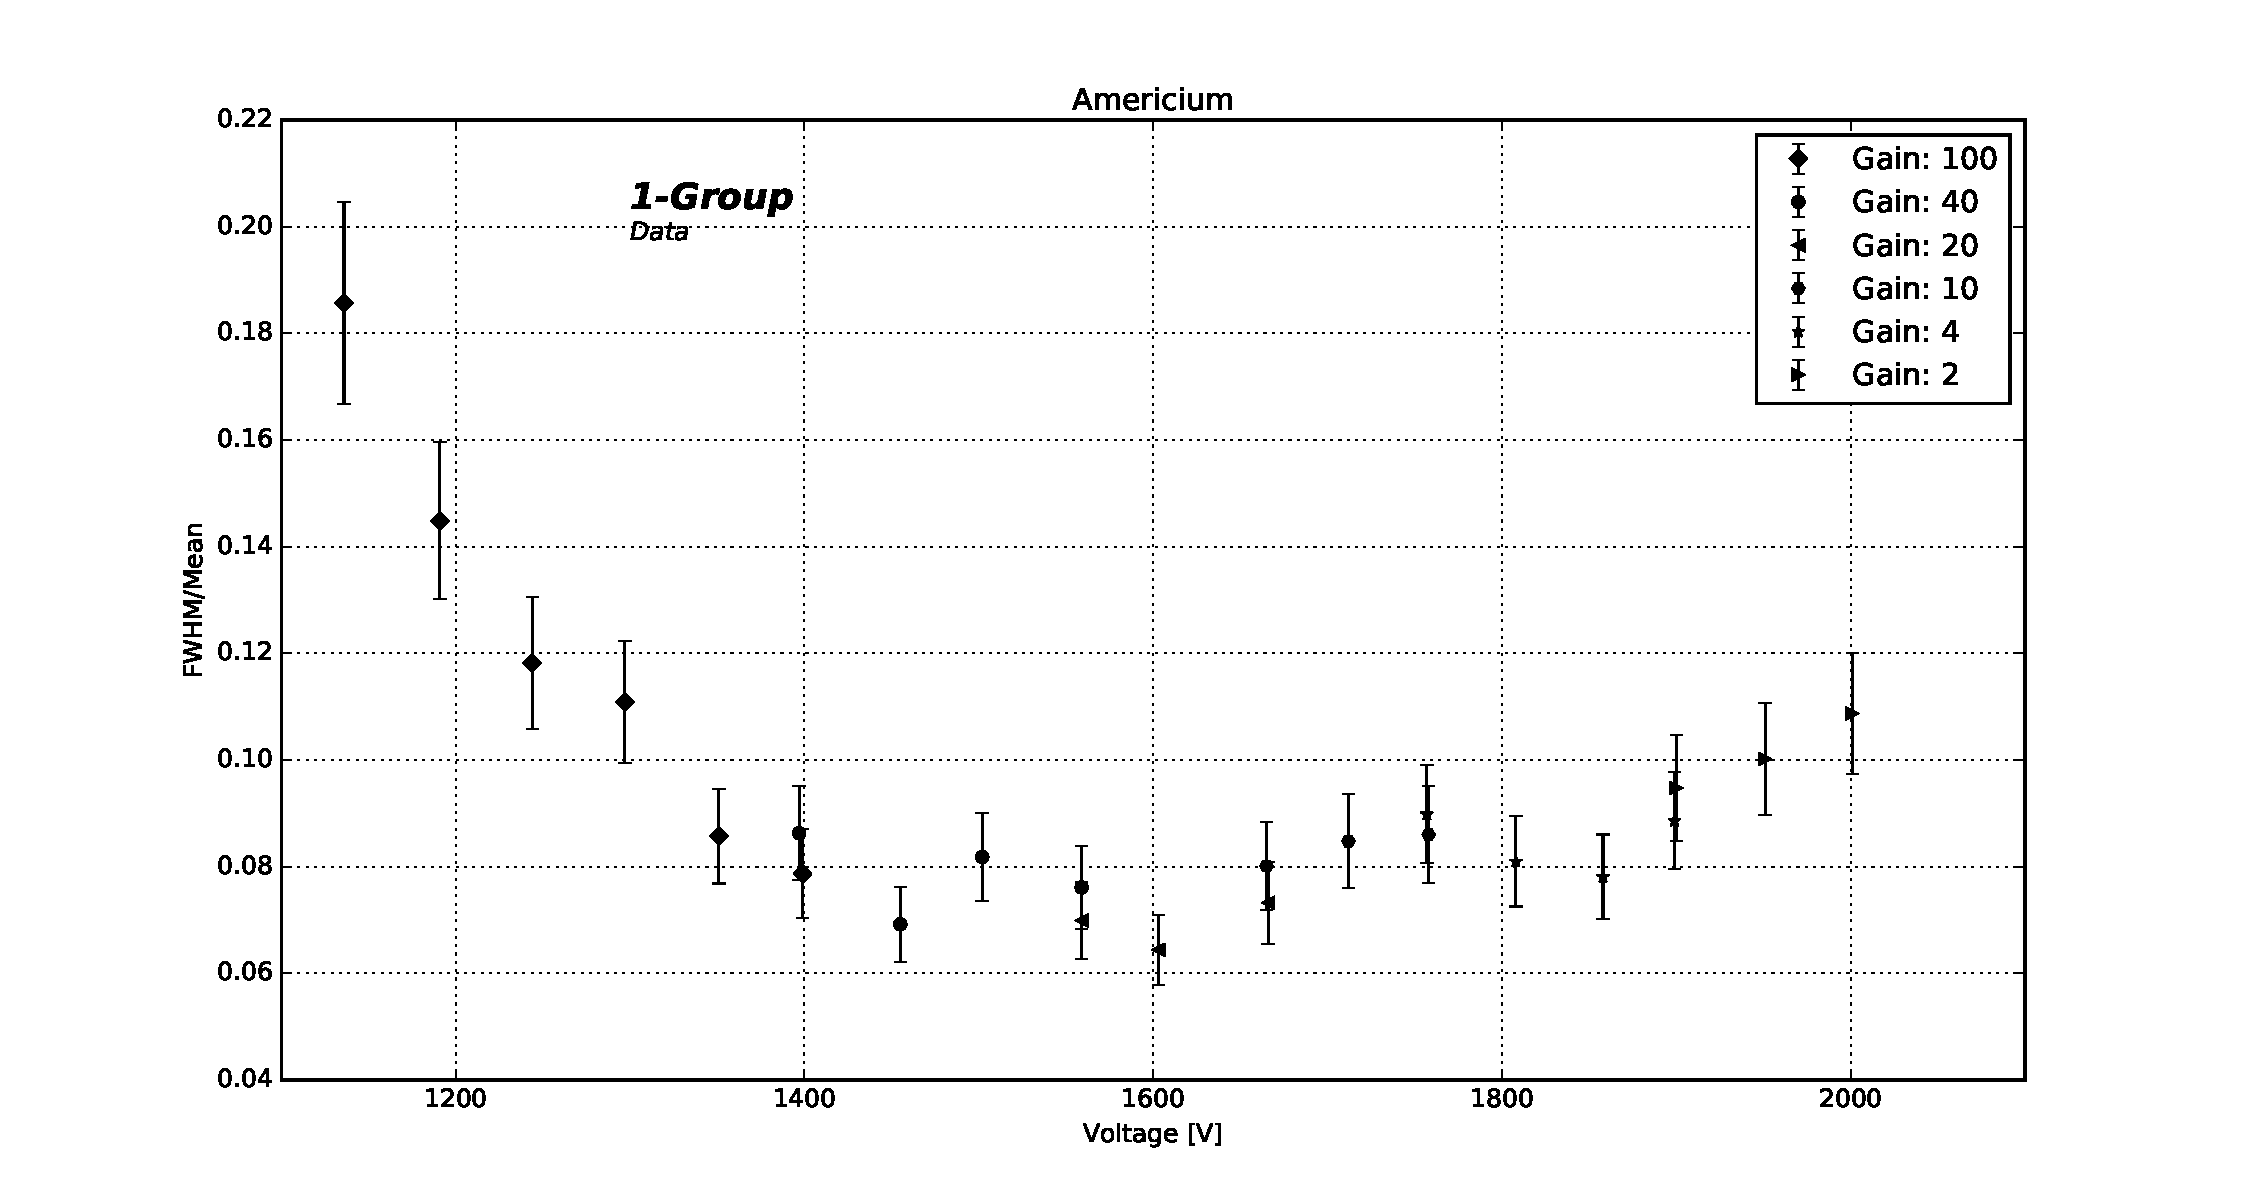
\includegraphics[width=\linewidth]{graphics/americium_scan}
  \caption{Americium scan}
  \label{fig:resolution:americium}
\end{figure}

\begin{figure}[htb]
  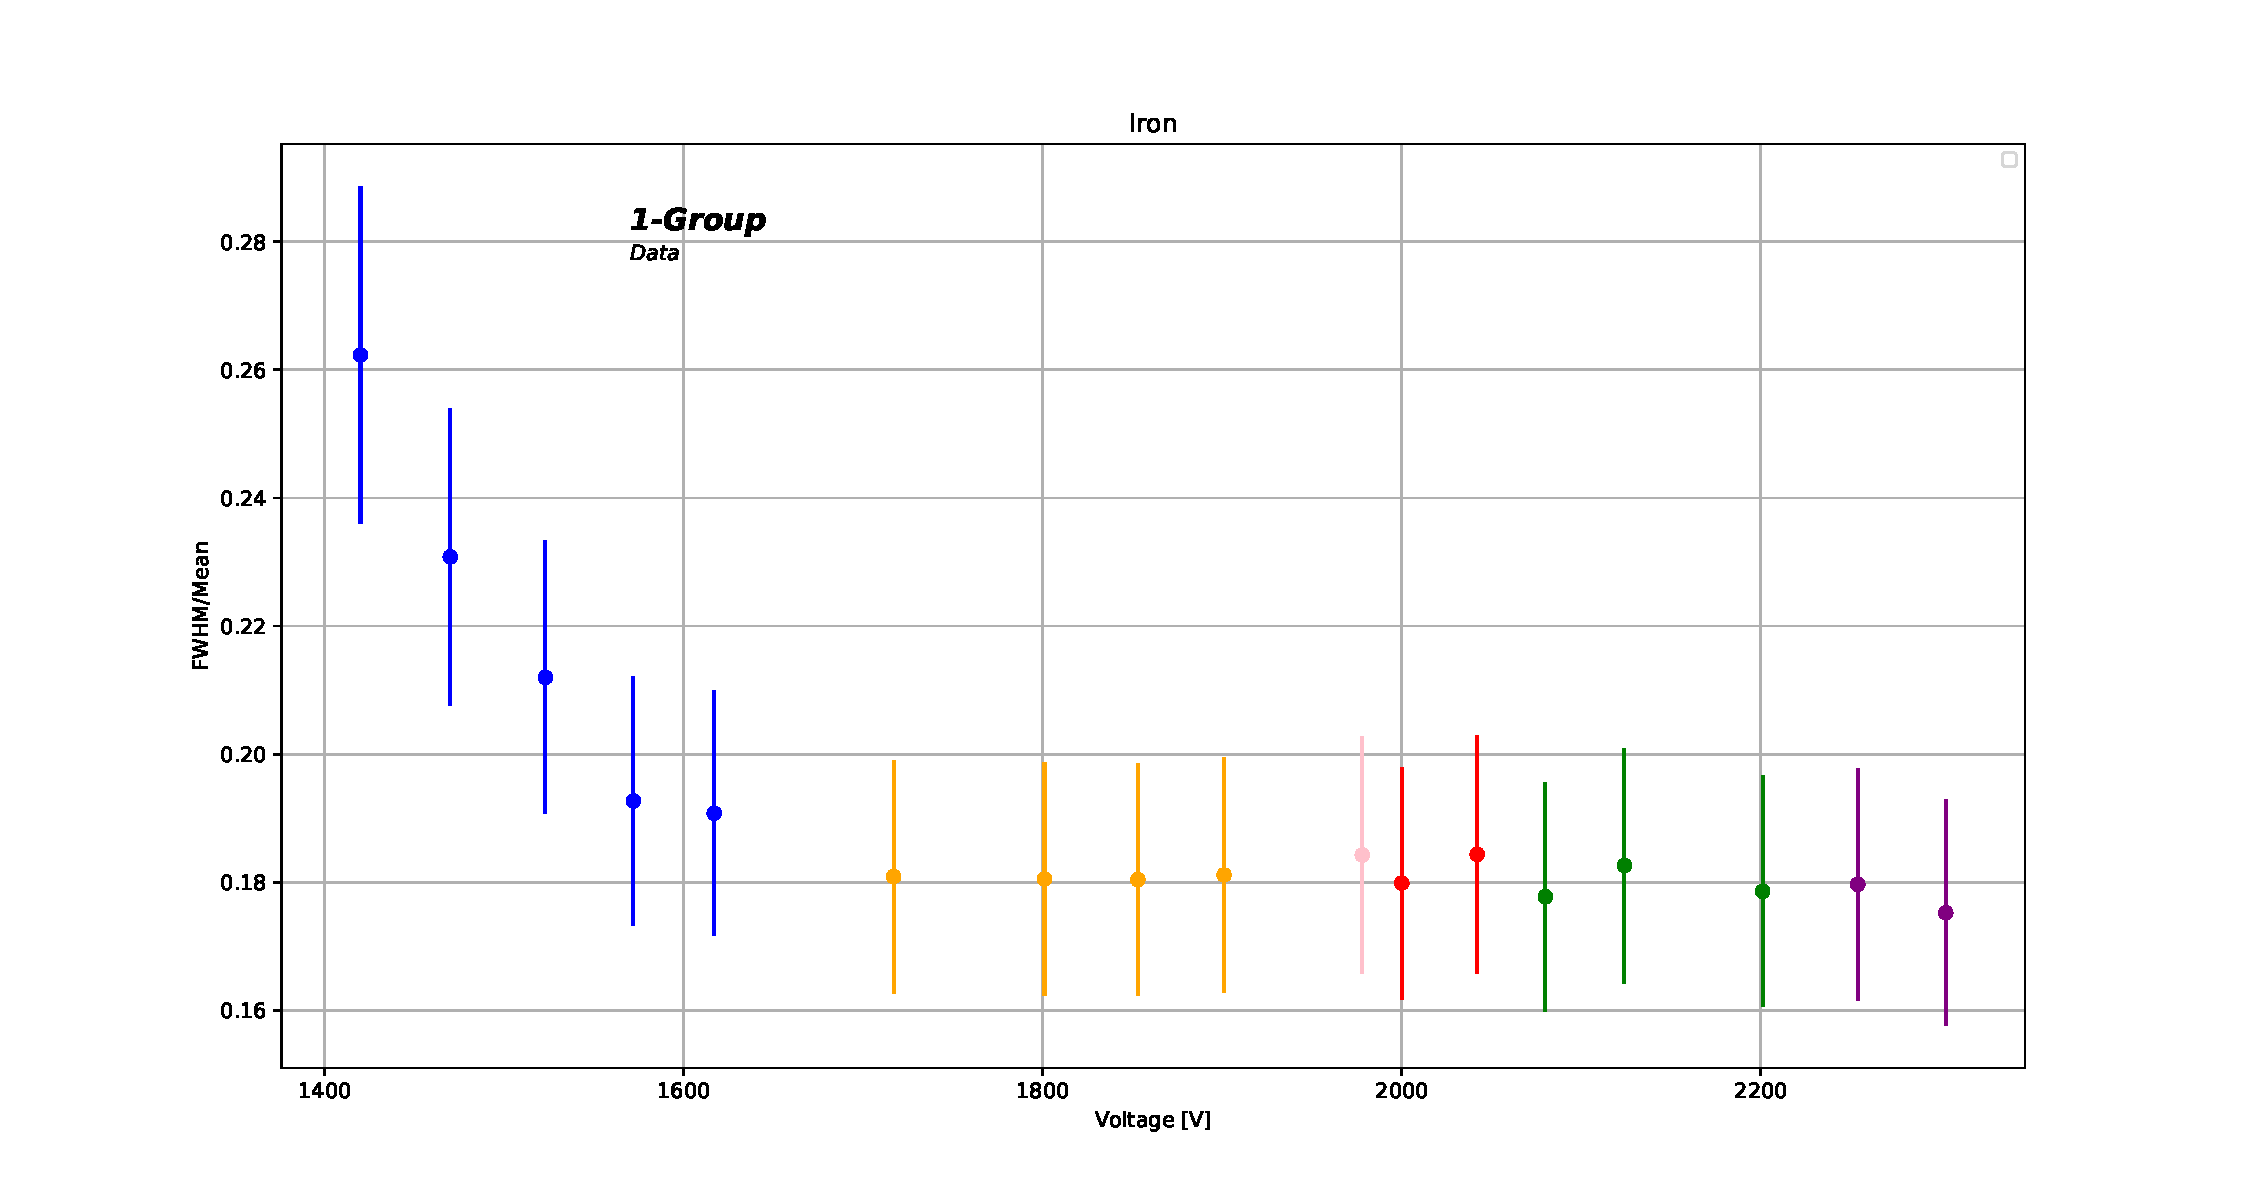
\includegraphics[width=\linewidth]{graphics/iron_scan}
  \caption{Iron scan}
  \label{fig:resolution:iron}
\end{figure}


%%%%%%%%%%%%%%%%%%%%%%%%%%%%%%%%%%%%%%%%%%%%
% Charge multiplication
%%%%%%%%%%%%%%%%%%%%%%%%%%%%%%%%%%%%%%%%%%%%

\section{Charge Multiplication}
\label{sec:systematics}

In the analysis of data from experiments, care must be taken to properly take into account systematic uncertainties in our measurements. In the case of the cider can detector, environmental and geometric factors can influence the overall performances of the drift chamber, namely the average number of carriers produced and collected at the electrodes. This number, called the \textit{gain} or \textit{multiplication factor}, can be approximated by the following formula, assuming that our detector is operating in the linear regime(\cite{gas_detect}):

\begin{adjustwidth}{+0.5cm}{}
\begin{align}
\ln(M)=\frac{\ln(2)}{\ln(r_{c}/r_{a})}\cdot\frac{V}{\Delta V}\cdot\ln\left[ \frac{V\rho_{o}}{ra\ln(r_{c}/r_{a})E_{min}(\rho_{o})\rho}\right]
\label{eq:lnm}
\end{align}
\end{adjustwidth}

The meaning and values associated with each parameter of this equation is listed in Tab. \ref{Tab:params}. One can see that most of these values either come from tabulated properties of the gas used, or are derived from the initial measurement of the beer can dimensions, listed in Tab. \ref{Tab:cidercan_sizes} for reference.

\begin{table*}[htb]
  \begin{tabularx}{\linewidth}{p{1.5cm}p{8cm}rl}
    \textbf{Variable}     & \textbf{Definition}                                                         & \textbf{Value}     & \textbf{Source}  \\
    \hline
    $r_{c}$                 & radius of the cathode                                                       & $3.121 \pm 0.003$      & Eq. \ref{eq:rcra}   \\
    &&&\\
    $r_{a}$                 & radius of the anode                                                         & $\SI{25 +- 2}{\micro\meter}$ & Eq. \ref{eq:rcra}   \\
    &&&\\
    $V$                    & operating voltage                                                           & 1-3 kV             & N/A                \\
    &&&\\
    $\Delta V$             & potential required to produce an additional electron                & $23.6 \pm 5.4$ V   &\cite{gas_detect}   \\
    &&&\\
    $E_{min}(\rho_{o})$      & \begin{tabular}[c]{@{}l@{}}Minimal electric field needed for ionisation\\(at standard pressure)\end{tabular}         & $48. \pm 3$ kV/cm  &\cite{gas_detect}   \\
    &&&\\
    $\rho_{o}/\rho$ & \begin{tabular}[c]{@{}l@{}}Standard density of the gas\\(compared to density at  T=273K and P = 1 bar)\end{tabular}  &                    &Eq. \ref{eq:gaslaw}, \cite{meteo}\\
    \hline
  \end{tabularx}
  \caption{List of the main systematics sources}
  \label{Tab:params}
\end{table*}

For the geometric properties, the relationship between the measured quantities and the anode radius, is simply $r_{a} = d_{a}/2.$. Meanwhile, the radii of the cathode is related to the other measurements via Eq. \ref{eq:rcra}.

\begin{align}
  \label{eq:rcra}
  r_{c} = \frac{D_{outer}}{2}-\tau
\end{align}

To determine the gas properties at the environmental conditions of the laboratory, one needed to measure the temperature and pressure of the room. With these values on hand, the ratio of gas densities can be determined by using the ideal gas law.

\begin{align}
  \label{eq:gaslaw}
  \frac{\rho}{\rho_{o}} = \frac{P}{P_{o}}\cdot \frac{T_{o}}{T}
\end{align}

During the measurements, the temperature stayed mostly constant, but the pressure varied over the course of the day, as shown in Fig. \ref{fig:pressure}. The uncertainty on the pressure was thus selected to be the largest pressure change with respect to standard pressure, over the course of a day.

\begin{figure}[htb]
  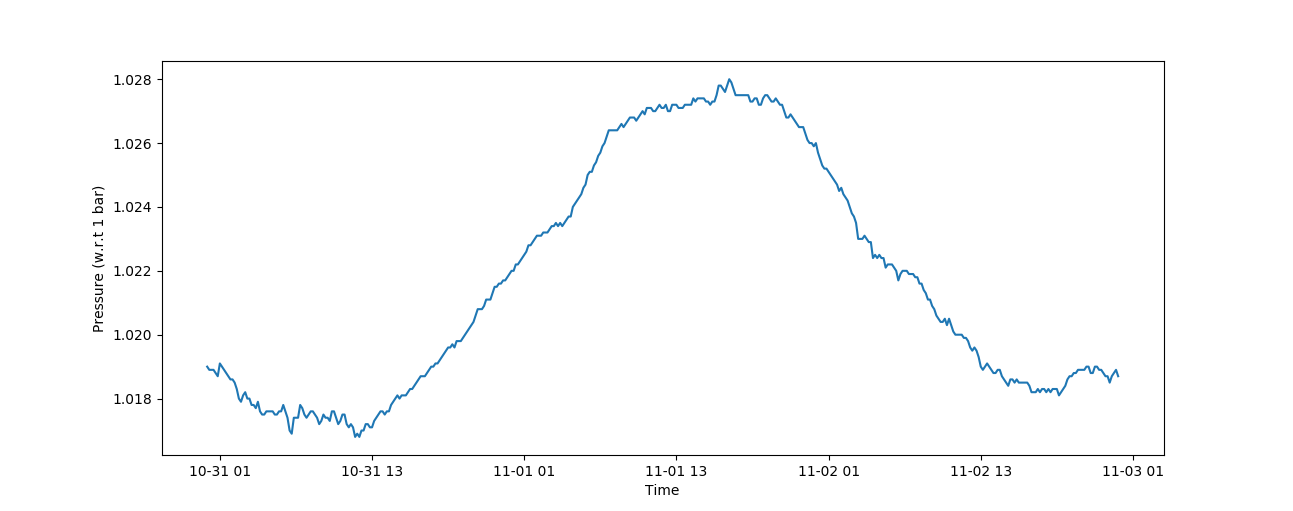
\includegraphics[width=0.5\textwidth]{graphics/pressure_monitoring.png}
  \caption{Atmospheric pressure in Helsinki during the spectra measurement. Source: \cite{meteo}}
  \label{fig:pressure}
\end{figure}

Given the parameters and uncertainties quoted in Tab. \ref{Tab:params}, a MC simulation was created in order to compute the theoretical uncertainties on the expected multiplication factor as a function of operating voltage. In this systematics treatment, each parameter was drawn out of Gaussian shaped probability distribution, with a mean centred at a parameter's value and the width set as the quoted uncertainty. Fig. \ref{final_lnm} shows the 1$\sigma$ and 2$\sigma$ confidence interval of the multiplication factor, after propagation of systematic uncertainties.

The theoretical expectation for the drift chamber's electron yield can be compared to the data obtained during the iron spectrum scan described in Sec. \ref{sec:resolution_scans}. Given a number of MCA counts $Q_{mca}$, the charge accumulated at the electrodes of the drift chamber can be obtained with Eq. \ref{eq:M_exp}.

\begin{align}
  \label{eq:M_exp}
  Q_{detector} = \frac{Q_{MCA}}{G_{pre,mca}\cdot{G_{coarse}}}
\end{align}

where $G_{pre,mca}$ is the preamplifier gain in units of $d.c./V$ (as plotted in Fig. \ref{fig:preamp_gain_mca}),and $G_{coarse}$ is the coarse gain that was described and measured in section \ref{sec:coarse}. From that point, the multiplication factor of the experimental data is given by Eq. \ref{eq:Mexp}.

\begin{align}
  \label{eq:Mexp}
  M_{experimental} &= \frac{N_{carriers,out}}{N_{carriers per avalanche}} \nonumber \\
                   &= \frac{Q_{detector}}{n_{Fe^{5},Am^{241}}\cdot e}
\end{align}

Where $n_{Fe^{55},Am^{241}}$ is the average number of electrons-ion pairs produced by either Fe$^{55}$ (227) or Am$^{241}$ (2290), as taken from \cite{can_paper}. The measured multiplication factors obtained in each voltage scan is shown in Fig. \ref{final_lnm}, along with the theoretical expectation for their values given the geometry of the can detector and the environmental conditions during the measurement. As one can see, the data collected is matches remarkably well the prediction, which has its $1\sigma$ and $2\sigma$ contours plotted in blue.

\begin{figure}[htb]
  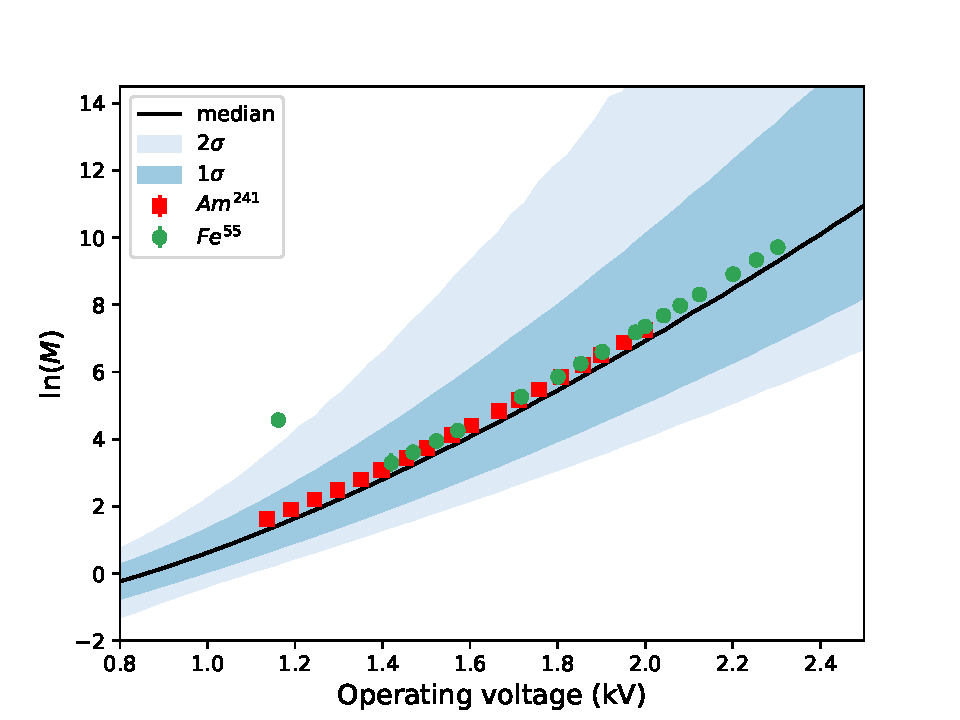
\includegraphics[width=0.5\textwidth]{graphics/lnM_final_plot.pdf}
  \caption{Natural logarithm of the drift chamber's multiplication factor M. Red and green data points represent the results obtained with $Fe^{55}$ and $Am^{241}$ respectively. Blue bands show the theoretical expectation for the detector, given systematics uncertainties in the cider can geometry and gas properties.}
  \label{final_lnm}
\end{figure}
